\documentclass[11pt]{article}

% ----------------------------------------------------------------------------
% ProPS-Twin -- Researcher-Facing Supporting Document (Document 1)
% Accessible companion to the "ProPS-Twin // live estate" HTML visualization.
% Every claim is grounded in the implementation (file:line where it matters).
% ----------------------------------------------------------------------------

\usepackage[utf8]{inputenc}
\usepackage[T1]{fontenc}
\usepackage{lmodern}
\usepackage[a4paper,margin=1in]{geometry}
\usepackage{microtype}
\usepackage{xcolor}
\usepackage{graphicx}
\usepackage{booktabs}
\usepackage{array}
\usepackage{longtable}
\usepackage{ragged2e}
\setlength{\emergencystretch}{3em}
\usepackage{amsmath}
\usepackage{amssymb}
\usepackage{enumitem}
\usepackage{tikz}
\usetikzlibrary{arrows.meta,positioning,shapes.geometric,fit,backgrounds,calc}
\usepackage{fancyhdr}
\usepackage[hidelinks]{hyperref}
\usepackage{titlesec}

% --- Moonfly-inspired accent palette (muted for print) ----------------------
\definecolor{mfbg}{HTML}{1c1c1c}
\definecolor{mfpurple}{HTML}{7a3fa0}
\definecolor{mfgreen}{HTML}{3a7d2c}
\definecolor{mfblue}{HTML}{2c4fb0}
\definecolor{mfcyan}{HTML}{127a6e}
\definecolor{mfred}{HTML}{b03030}
\definecolor{mfyellow}{HTML}{8a6d12}
\definecolor{mfgray}{HTML}{555555}
\definecolor{panel}{HTML}{f2f2f2}
\definecolor{panelline}{HTML}{cccccc}

\hypersetup{colorlinks=true,linkcolor=mfblue,urlcolor=mfblue,citecolor=mfblue}

% inline code helper (underscores inside must be escaped as \_ )
\newcommand{\code}[1]{\texttt{\small #1}}
\newcommand{\file}[1]{\textcolor{mfpurple}{\texttt{\small #1}}}

\titleformat{\section}{\Large\bfseries\color{mfpurple}}{\thesection}{0.6em}{}
\titleformat{\subsection}{\large\bfseries\color{mfblue}}{\thesubsection}{0.6em}{}

\pagestyle{fancy}
\fancyhf{}
\lhead{\small\textcolor{mfgray}{ProPS-Twin -- Researcher Guide}}
\rhead{\small\textcolor{mfgray}{\thepage}}
\renewcommand{\headrulewidth}{0.3pt}

\newcommand{\keyfact}[1]{%
  \par\vspace{4pt}\noindent
  \colorbox{panel}{\parbox{\dimexpr\linewidth-2\fboxsep}{\small\textbf{\textcolor{mfcyan}{Verified:}} #1}}%
  \par\vspace{4pt}}

% ============================================================================
\begin{document}

\begin{titlepage}
\centering
\vspace*{2cm}
{\color{mfpurple}\rule{\linewidth}{1.2pt}}\\[8pt]
{\Huge\bfseries ProPS-Twin}\\[6pt]
{\LARGE A Researcher's Guide to the\\ Live Estate Visualization}\\[10pt]
{\color{mfpurple}\rule{\linewidth}{1.2pt}}\\[14pt]
{\large An accessible, implementation-grounded companion to the\\
\emph{``ProPS-Twin // live estate''} browser interface}\\[1.2cm]

\begin{tabular}{rl}
\textbf{System} & LLM-guided IT/OT security digital twin\\
\textbf{Evaluator} & Log-only (fast-mode), offline detection\\
\textbf{Estate} & 5 simulated components across 4 zones\\
\textbf{Scenarios} & SC-01 \ldots SC-07\\
\textbf{Reward} & $R = w_dD + w_cC + w_aA + w_rQ - w_fF - w_lL$\\
\textbf{Status} & Local simulation path implemented \& tested (48 tests pass)\\
\end{tabular}

\vfill
{\small This document explains \emph{what you are looking at} in the visualization,
where every number comes from, and how the data travels from a simulated device
all the way to the screen. It assumes a research or machine-learning background
but \emph{no} prior knowledge of industrial-control security.}\\[6pt]
{\small\color{mfgray}Generated from the verified implementation at
\file{/CSE499} on 2026-11-19.}
\end{titlepage}

\tableofcontents
\clearpage

% ============================================================================
\section{What ProPS-Twin is, in one minute}

ProPS-Twin is a \textbf{digital twin}: a small, self-contained software model of
the security-monitoring estate of an industrial facility (the running example is
a nuclear power plant's IT/OT environment, where \emph{IT} means ordinary office
and business networks and \emph{OT} means the operational technology that runs
the physical process). Instead of attacking a real plant, the twin
\emph{simulates} five networked components, injects a controlled security
incident into them, writes out exactly the kind of log events those components
would emit, and then scores how well a security policy would have coped --- all
on a laptop, with no cluster and no real traffic.

The long-term research goal is to let a large language model propose and refine
defensive \emph{policies} (``prompted policy search'') and measure each policy
with a single, honest \textbf{reward} number. The visualization you are reading
about is the window into one run of that loop: it shows the estate reacting, the
raw event stream scrolling past, and the reward being assembled from its parts.

\keyfact{The entire simulation-and-scoring path runs on the Python standard
library alone --- no web framework, no scientific stack, no external services.
See \file{research/}, \file{services/}, and \file{scripts/}.}

\subsection{The three things the interface shows you}

\begin{enumerate}[leftmargin=1.4em]
  \item \textbf{The estate} --- five components, grouped by security zone,
        lighting up as they emit events.
  \item \textbf{The event stream} --- the raw JSON-lines telemetry, formatted
        like a terminal log, exactly as it would appear on \code{stdout}.
  \item \textbf{The reward} --- one score $R$ and the six measured dimensions
        it is built from, updated at the end of the run.
\end{enumerate}

Everything else on the page (the timeline, the controls, the counters) exists to
give those three things context.

% ============================================================================
\section{The system at a glance}
\label{sec:architecture}

Figure~\ref{fig:arch} is the map. Read it left to right: a scenario definition
drives five component models; the Scenario Controller steps a virtual clock and
collects every event they emit; that event stream is the \emph{only} thing the
evaluator sees; the evaluator turns it into a reward document; and a thin backend
streams the whole thing to the browser.

\begin{figure}[h]
\centering
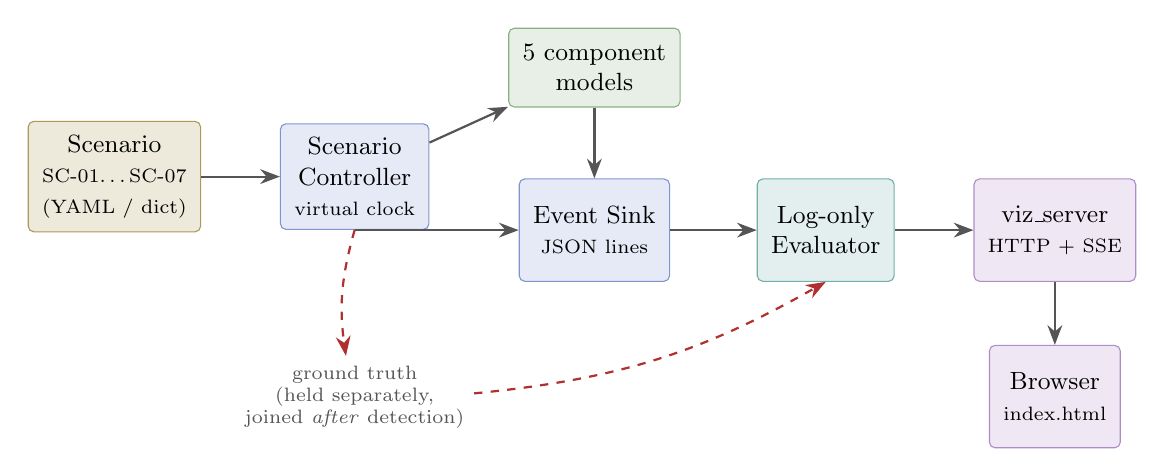
\begin{tikzpicture}[
  font=\small,
  box/.style={rectangle,rounded corners=2pt,draw=panelline,fill=panel,
              minimum height=1.0cm,align=center,inner sep=5pt},
  comp/.style={box,fill=mfgreen!12,draw=mfgreen!60},
  core/.style={box,fill=mfblue!12,draw=mfblue!60,minimum height=1.3cm},
  eval/.style={box,fill=mfcyan!12,draw=mfcyan!60,minimum height=1.3cm},
  ui/.style={box,fill=mfpurple!12,draw=mfpurple!60,minimum height=1.3cm},
  arr/.style={-{Stealth[length=2.5mm]},thick,draw=mfgray},
  ]
  \node[box,fill=mfyellow!15,draw=mfyellow!70] (sc) {Scenario\\\scriptsize SC-01\ldots SC-07\\\scriptsize (YAML / dict)};
  \node[core,right=1.0cm of sc] (ctrl) {Scenario\\Controller\\\scriptsize virtual clock};
  \node[comp,above right=0.2cm and 1.0cm of ctrl] (c1) {5 component\\models};
  \node[core,below=0.9cm of c1] (sink) {Event Sink\\\scriptsize JSON lines};
  \node[eval,right=1.1cm of sink] (ev) {Log-only\\Evaluator};
  \node[ui,right=1.0cm of ev] (back) {viz\_server\\\scriptsize HTTP + SSE};
  \node[ui,below=0.8cm of back] (html) {Browser\\\scriptsize index.html};

  \draw[arr] (sc) -- (ctrl);
  \draw[arr] (ctrl) -- (c1);
  \draw[arr] (c1) -- (sink);
  \draw[arr] (ctrl.south) |- (sink.west);
  \draw[arr] (sink) -- (ev);
  \draw[arr] (ev) -- (back);
  \draw[arr] (back) -- (html);
  \node[below=1.6cm of ctrl,align=center,text=mfgray,font=\scriptsize]
      (gt) {ground truth\\(held separately,\\joined \emph{after} detection)};
  \draw[arr,dashed,draw=mfred] (ctrl.south) to[bend right=12] (gt);
  \draw[arr,dashed,draw=mfred] (gt) to[bend right=12] (ev.south);
\end{tikzpicture}
\caption{The data path. Solid arrows carry telemetry; the dashed red path is the
ground truth, which is deliberately kept \emph{out} of the event stream and only
matched to alerts after detection has happened (Section~\ref{sec:honest}).}
\label{fig:arch}
\end{figure}

\subsection{Who produces what}

\begin{longtable}{>{\RaggedRight\arraybackslash}p{2.6cm} >{\RaggedRight\arraybackslash}p{3.4cm} >{\RaggedRight\arraybackslash}p{7.4cm}}
\toprule
\textbf{Stage} & \textbf{Code} & \textbf{Responsibility}\\
\midrule
\endhead
Scenario & \file{configs/scenarios/}, \file{catalog.py}
  & Defines the seed, the incident to inject, its time window, and the ground
    truth (what \emph{should} be detected).\\
Components & \file{services/*/core.py}
  & Five device models. Each produces one JSON event per tick describing what it
    ``sees'' --- normal heartbeats most of the time, incident telemetry when the
    scenario puts it in an attack mode.\\
Controller & \file{controller.py}
  & Builds the components, advances a virtual clock second by second, flips modes
    on schedule, and collects every emitted event.\\
Event Sink & \file{props\_log.py}
  & Stamps each event with a deterministic ID and timestamp and writes it as a
    JSON line (the same text a real container would log).\\
Evaluator & \file{engine.py}, \file{metrics.py}
  & Re-derives detections from the telemetry alone, matches them to ground truth,
    and computes the six reward dimensions and the final $R$.\\
Backend & \file{viz\_server.py}
  & A standard-library HTTP server that runs a scenario on request and streams it
    to the browser over Server-Sent Events (SSE).\\
Interface & \file{viz/index.html}
  & Renders the estate, the event log, the timeline, and the reward dashboard.\\
\bottomrule
\end{longtable}

% ============================================================================
\section{The data lifecycle: following one event}
\label{sec:lifecycle}

It helps to follow a single event on its journey. Suppose we run \textbf{SC-01},
the scenario in which a non-whitelisted protocol crosses the IDMZ boundary.

\begin{enumerate}[leftmargin=1.5em]
  \item \textbf{Origin.} At simulated second $t=30$ the controller puts the
        \code{idmz-gateway} component into the mode
        \code{inter\_zone\_protocol\_anomaly}. On that tick the gateway's
        \code{tick()} method emits an event: event type
        \code{inter\_zone\_protocol\_anomaly}, severity \code{high}, simulated
        state \code{anomalous}, and a details payload containing a
        \code{drop\_rate} that has been bumped up by $0.20$ above its quiet
        baseline (\file{services/idmz\_gateway/core.py}).
  \item \textbf{Stamping.} The event passes through the Event Sink, which adds a
        timestamp from the virtual clock and a \emph{deterministic} event ID ---
        a SHA-256 hash of \code{experiment|component|sequence} --- so the exact
        same run always produces the exact same IDs
        (\file{props\_log.py}, \code{deterministic\_event\_id}).
  \item \textbf{Transport.} The sink writes the event as one line of JSON to
        \code{stdout} (and keeps a copy in memory). This is the text you see in
        the \emph{event stream} panel.
  \item \textbf{Detection.} When the run finishes, the evaluator looks at the
        raw events \emph{without ever consulting the ground truth}. For a signal
        that carries a \code{drop\_rate}, it fires an alert when the rate crosses
        a cutoff set by the \code{alert\_threshold} policy; for events with no
        rate, it fires when the state is \code{anomalous}, \code{fault}, or
        \code{violation}. Our bumped drop-rate sails past the cutoff, so an alert
        is raised (\file{engine.py}, \code{detect\_presence}).
  \item \textbf{Matching.} Only now does the evaluator open the ground-truth
        table. The alert's event ID falls inside the labelled window
        $[30,50]$ for the \code{idmz-gateway}, so it is counted as a
        \textbf{true positive}.
  \item \textbf{Scoring.} True positives, false positives, missed positives,
        containment flags, availability probes, and recovery times are rolled up
        into the six dimensions $D, C, A, Q, F, L$ and combined into the reward
        $R$ (\file{metrics.py}).
  \item \textbf{Display.} The backend streams each tick to the browser as it is
        replayed, then sends the final reward document; the dashboard fills in
        the score, the six bars, and the counters.
\end{enumerate}

Figure~\ref{fig:lifecycle} shows this as a pipeline.

\begin{figure}[h]
\centering
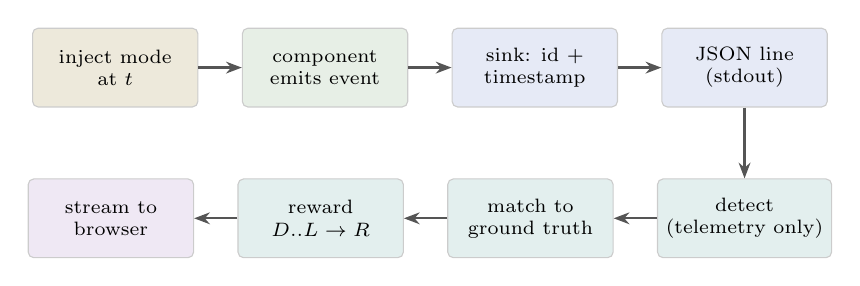
\begin{tikzpicture}[
  font=\scriptsize,node distance=0.55cm,
  stage/.style={rectangle,rounded corners=2pt,draw=panelline,fill=panel,
                minimum width=2.1cm,minimum height=1.0cm,align=center,inner sep=3pt},
  arr/.style={-{Stealth[length=2mm]},thick,draw=mfgray},
  ]
  \node[stage,fill=mfyellow!15] (a) {inject mode\\at $t$};
  \node[stage,fill=mfgreen!12,right=of a] (b) {component\\emits event};
  \node[stage,fill=mfblue!12,right=of b] (c) {sink: id +\\timestamp};
  \node[stage,fill=mfblue!12,right=of c] (d) {JSON line\\(stdout)};
  \node[stage,fill=mfcyan!12,below=0.9cm of d] (e) {detect\\(telemetry only)};
  \node[stage,fill=mfcyan!12,left=of e] (f) {match to\\ground truth};
  \node[stage,fill=mfcyan!12,left=of f] (g) {reward\\$D..L \to R$};
  \node[stage,fill=mfpurple!12,left=of g] (h) {stream to\\browser};
  \draw[arr] (a)--(b); \draw[arr] (b)--(c); \draw[arr] (c)--(d);
  \draw[arr] (d)--(e); \draw[arr] (e)--(f); \draw[arr] (f)--(g); \draw[arr] (g)--(h);
\end{tikzpicture}
\caption{One event's path from injection to the screen. Detection (bottom row,
right to left) is computed from telemetry before ground truth is ever consulted.}
\label{fig:lifecycle}
\end{figure}

% ============================================================================
\section{The five estate components}
\label{sec:components}

The estate is five device models, each living in a security \emph{zone}. Zones
are concentric trust rings: the further from the plant floor, the less trusted.
Table~\ref{tab:components} lists them in the order the interface stacks them.

\begin{table}[h]
\centering
\caption{The simulated estate. Each component is a Python class in
\file{services/<name>/core.py} with a \code{tick()} method that emits one or
more events per simulated second.}
\label{tab:components}
\small
\begin{tabular}{p{3.0cm} p{2.0cm} p{8.3cm}}
\toprule
\textbf{Component} & \textbf{Zone} & \textbf{What it models \& which scenarios touch it}\\
\midrule
idmz-gateway & idmz
  & Brokers traffic between zones at the industrial DMZ boundary. Emits
    protocol-anomaly, jump-host-crossing, and unauthenticated-access signals.
    Drives SC-01, SC-04, SC-06.\\
boundary-firewall & idmz
  & Enforces the protocol whitelist and rate limits. Emits drop-rate and
    packet-storm signals. Drives SC-02.\\
plc-edge & field
  & A programmable logic controller at the plant floor. Emits a watchdog
    heartbeat every tick plus firmware-integrity status.\\
eng-station & supervisory
  & An engineering workstation. Emits a compliance status and a periodic
    security-audit log, plus privileged-command events. Drives SC-03, SC-05.\\
telemetry-forwarder & control
  & A one-way data diode forwarding telemetry out of the plant. Emits forwarding
    health and answers availability probes. Drives SC-07.\\
\bottomrule
\end{tabular}
\end{table}

\keyfact{The interface groups components under four zone headers --- \emph{idmz,
supervisory, control, field} --- matching \code{ZONE\_ORDER} in \file{index.html}
and \code{COMPONENT\_ZONE} in \file{controller.py}. A fifth logical zone,
\emph{enterprise}, exists in the schema as the source of some crossings but has
no component of its own.}

\subsection{How a component behaves during an incident}

Every component spends most of its time in \code{normal} mode, emitting quiet
heartbeats. Some of those heartbeats are deliberate \textbf{near-misses}: once
every few ticks the drop-rate is nudged up a little (but not past the alert
cutoff at the default threshold). These exist so that a careless, over-sensitive
policy will start raising \emph{false positives} on them --- which is exactly
what makes the reward move when you lower the alert threshold.

When the scenario injects an incident, the component switches to an attack mode
and emits the incident telemetry instead. Two components also carry a
\code{contained} flag whose value depends on the \emph{access profile} policy:
under \code{strict} or \code{lockdown} the device blocks the malicious crossing
itself (``contained''), and under \code{standard} it does not. That single flag
is what the containment dimension $C$ measures.

% ============================================================================
\section{The seven scenarios (these are \emph{not} the metrics)}
\label{sec:scenarios}

A common confusion is to mix up the \textbf{seven scenarios} with the
\textbf{six evaluation dimensions}. They are different things:

\begin{itemize}[leftmargin=1.4em]
  \item A \textbf{scenario} (SC-01 \ldots SC-07) is one \emph{situation}: a
        specific incident injected into a specific component at a specific time.
        It is the \emph{input} to a run.
  \item A \textbf{dimension} ($D, C, A, Q, F, L$) is one \emph{way of measuring}
        how a run went. It is part of the \emph{output}.
  \item Every scenario is scored on all six dimensions; most dimensions are
        simply ``not applicable'' (and score a neutral $1.0$) for scenarios that
        do not exercise them.
\end{itemize}

Table~\ref{tab:scenarios} is the catalog. Each scenario's full anatomy follows.

\begin{table}[h]
\centering
\caption{The seven scenarios, from \file{configs/scenarios/} and
\file{catalog.py}. ``Type'' is the detection style: \emph{presence} (something
bad appears) or \emph{absence} (something required goes missing).}
\label{tab:scenarios}
\scriptsize
\begin{tabular}{p{1.0cm} p{3.1cm} p{2.0cm} p{1.3cm} p{1.1cm} p{3.0cm}}
\toprule
\textbf{ID} & \textbf{Incident} & \textbf{Component} & \textbf{Window} & \textbf{Type} & \textbf{Primary dimension tested}\\
\midrule
SC-01 & Non-whitelisted inter-zone protocol & idmz-gateway & $[30,50]$ & presence & Detection\\
SC-02 & Broadcast/multicast packet storm & boundary-firewall & $[40,55]$ & presence & Detection + containment\\
SC-03 & Privilege escalation & eng-station & $[50,51]$ & presence & Containment (uncontained at baseline)\\
SC-04 & Zone-segmentation violation & idmz-gateway & $[35,45]$ & presence & Containment (policy lever)\\
SC-05 & Missing security-audit log & eng-station & $[40,70]$ & absence & Coverage + delay\\
SC-06 & Unauthenticated remote access & idmz-gateway & $[45,53]$ & presence & Containment\\
SC-07 & Forwarding heartbeat pause, then recovery & telemetry-forwarder & $[40,60]$ & absence & Availability + recovery\\
\bottomrule
\end{tabular}
\end{table}

\subsection{SC-01 --- Non-whitelisted inter-zone protocol}
\textbf{Purpose:} the baseline presence case --- can the pipeline detect a clearly
anomalous crossing? \textbf{Input / trigger:} at $t=30$ the \code{idmz-gateway}
enters \code{inter\_zone\_protocol\_anomaly} for 20 seconds. \textbf{Flow:} the
gateway emits one anomalous event per tick with an elevated drop-rate.
\textbf{Expected behaviour:} every tick in $[30,50]$ is an alert.
\textbf{Observed output:} 20 true positives, no false positives.
\textbf{Evaluation:} detection rate $D$. \textbf{Interpretation:} $R=0.85$ ---
the maximum achievable --- because every reward dimension is satisfied.

\subsection{SC-02 --- Broadcast/multicast packet storm}
\textbf{Purpose:} detect a volumetric anomaly \emph{and} test whether the firewall
contains it. \textbf{Trigger:} at $t=40$ the \code{boundary-firewall} enters
\code{packet\_storm} for 15 seconds. \textbf{Flow:} each tick emits \emph{two}
events --- a packet-storm-volume reading and a boundary-drop-rate reading --- both
far above the cutoff. The storm is marked \code{contained} because the rate limit
($50$) is at or below the containment threshold ($60$). \textbf{Observed:} 15 true
positives (from 30 alerts), containment $=1.0$. \textbf{Interpretation:} $R=0.85$.

\subsection{SC-03 --- Privilege escalation}
\textbf{Purpose:} show a correctly-\emph{detected} but \emph{uncontained} incident.
\textbf{Trigger:} at $t=50$ the \code{eng-station} executes a privileged command
(1-second window). \textbf{Flow:} one violation event carrying a \code{contained}
flag; at the baseline \code{standard} access profile that flag is \code{false}.
\textbf{Observed:} detection $D=1.0$, containment $C=0.0$. \textbf{Interpretation:}
$R=0.60$. The gap from $0.85$ to $0.60$ is exactly the containment weight
($w_c=0.25$) going unearned --- a vivid illustration that detection alone is not
enough.

\subsection{SC-04 --- Zone-segmentation violation}
\textbf{Purpose:} the headline policy-lever demonstration. \textbf{Trigger:} at
$t=35$ a jump-host crossing from enterprise toward control, for 10 seconds.
\textbf{Flow:} the gateway emits a violation per tick with a \code{contained} flag
driven by the access profile. \textbf{Observed:} at \code{standard}, $C=0.0$ and
$R=0.60$; at \code{strict} or \code{lockdown}, $C=1.0$ and $R=0.85$.
\textbf{Interpretation:} this is the scenario to run twice --- once per profile ---
to \emph{see} a policy change move the reward live. It is also the subject of a
dedicated regression test.

\subsection{SC-05 --- Missing security-audit log (absence)}
\textbf{Purpose:} detect something by its \emph{absence}. \textbf{Trigger:} at
$t=40$ the \code{eng-station} enters \code{audit\_log\_gap} for 30 seconds. The
host stays alive and keeps reporting compliance, but it \emph{stops} emitting the
required \code{security\_audit\_log}. \textbf{Flow:} the evaluator scans for the
longest stretch where the required periodic signal is missing; a gap longer than
the 5-second timeout raises a coverage alert. \textbf{Observed:} a 30-second gap
starting at $t=40$ is detected; $D=1.0$, but the delay penalty $L=0.042$ because
an absence takes the timeout (5 s) to confirm. \textbf{Interpretation:} $R=0.8479$
--- almost perfect, docked only by the unavoidable confirmation delay.

\subsection{SC-06 --- Unauthenticated remote access}
\textbf{Purpose:} a second containment case on the identity path. \textbf{Trigger:}
at $t=45$, an unauthenticated remote-access attempt for 8 seconds. \textbf{Flow:}
a violation per tick with a \code{contained} flag. \textbf{Observed:} $D=1.0$,
$C=0.0$ at baseline, $R=0.60$. \textbf{Interpretation:} like SC-03 and SC-04, the
baseline policy sees the attack but does not stop it.

\subsection{SC-07 --- Heartbeat pause, then recovery (absence + availability)}
\textbf{Purpose:} the richest scenario --- it exercises absence detection,
availability, \emph{and} recovery at once. \textbf{Trigger:} at $t=40$ the
\code{telemetry-forwarder} pauses its forwarding heartbeat for 20 seconds; when it
resumes it must drain a buffer before it is truly healthy. \textbf{Flow:} the
heartbeat gap is detected by absence; meanwhile an availability prober polls the
forwarder every 10 seconds and records failures while it is unavailable; the
recovery time is the settle delay after the fault window ends. \textbf{Observed:}
$D=1.0$, availability $A=0.75$ (9 of 12 probes succeed), recovery $Q=0.90$
(a 6-tick drain against a 60-second budget), $L=0.042$. \textbf{Interpretation:}
$R=0.7879$ --- the twin never ``crashes''; it degrades measurably and recovers
within budget, which is precisely what the availability and recovery dimensions
are designed to capture.

% ============================================================================
\section{The six evaluation dimensions and the reward}
\label{sec:metrics}

The reward is a single number that summarises a whole run:
\begin{equation}
R(\pi) = w_d D + w_c C + w_a A + w_r Q - w_f F - w_l L .
\label{eq:reward}
\end{equation}
Four terms are rewards (you want them high) and two are penalties (you want them
low). Table~\ref{tab:dims} defines each one and names the weight the interface
displays beside its bar.

\begin{table}[h]
\centering
\caption{The six dimensions, from \file{research/evaluation/metrics.py}. Each is
normalised to $[0,1]$. The weights are the \code{DEFAULT\_WEIGHTS} in that file
(identical to \file{configs/evaluation/reward.yaml}).}
\label{tab:dims}
\small
\begin{tabular}{c p{3.2cm} c p{6.7cm}}
\toprule
\textbf{Sym} & \textbf{Dimension} & \textbf{Weight} & \textbf{Meaning}\\
\midrule
$D$ & Detection rate & $0.30$ & Fraction of labelled incidents detected: $|TP|/|G|$.\\
$C$ & Containment & $0.25$ & Fraction of malicious attempts blocked before effect.\\
$A$ & Availability & $0.20$ & Fraction of legitimate availability probes answered in time.\\
$Q$ & Recovery & $0.10$ & $1-\min(1,t_\text{rec}/\text{budget})$: how quickly a fault settles.\\
$F$ & False-positive penalty & $0.10$ & Alerts raised on benign events, per benign event.\\
$L$ & Delay penalty & $0.05$ & Normalised mean detection delay; misses count as the full window.\\
\bottomrule
\end{tabular}
\end{table}

\keyfact{Because the four positive weights sum to $0.85$ and the penalties can at
best be zero, \textbf{the highest reachable reward is $0.85$} --- which is why the
dashboard prints the score ``\code{/ 0.85 max}''. SC-01 and SC-02 hit it exactly.}

\paragraph{Neutral defaults.} When a dimension does not apply to a scenario it
scores a neutral $1.0$ (for rewards) or $0.0$ (for penalties) rather than dragging
the reward down. For example SC-01 has nothing to contain, so $C=1.0$ by
convention; SC-03 has no availability probes, so $A=1.0$. These conventions are
documented in \file{metrics.py} and keep the reward comparable across scenarios.

\paragraph{One honest caveat about delay.} For \emph{presence} incidents the
implementation currently records a detection delay of exactly zero
(\file{engine.py}, the line
\code{matched\_delays.extend(0.0 for \_ in matched)}). In effect the log-only
evaluator treats an alert as instantaneous once the telemetry is available.
Only \emph{absence} incidents (SC-05, SC-07) carry a real delay, equal to the
coverage timeout. So wherever you see $L=0.042$ it is an absence confirmation
delay, and wherever you see $L=0$ on a presence scenario it reflects this
modelling choice, not a measured latency. This is worth knowing before drawing
conclusions about detection speed.

% ============================================================================
\section{Reading the interface, element by element}
\label{sec:interface}

This section walks the screen top to bottom. Every element named here is in
\file{viz/index.html}.

\subsection{Header and status badge}
The title reads \emph{``ProPS-Twin // live estate''} with the subtitle
\emph{``LLM-guided IT/OT security digital twin $\cdot$ log-only evaluator''}. The
badge at the top right is the single most important status indicator:
\begin{itemize}[leftmargin=1.4em,nosep]
  \item \textbf{live} (green dot) --- a backend was found; runs are \emph{fresh
        simulations} streamed in real time and the policy levers work.
  \item \textbf{offline} (yellow dot) --- no backend; the page replays
        \code{demo\_data.json}, a baked file of \emph{real} simulation output.
        The policy levers are locked because changing them would require
        re-simulating.
  \item \textbf{err} (red dot) --- neither a backend nor the demo file was found.
\end{itemize}
On start-up the page quietly tries three backend addresses before falling back to
the offline file, so the badge tells you which mode you ended up in.

\subsection{The control bar}
\begin{description}[leftmargin=1.4em,style=nextline]
  \item[scenario] picks which of SC-01\ldots SC-07 to run.
  \item[incident] a read-only description of the selected scenario's incident.
  \item[speed] how many simulated seconds to replay per wall-clock second
        ($2\times$ to $120\times$). It changes only the playback pace, never the
        result.
  \item[access profile] the containment lever: \emph{standard} (baseline),
        \emph{strict}, or \emph{lockdown}. Strict and lockdown block malicious
        crossings (raising $C$); lockdown additionally starves \emph{legitimate}
        probes (lowering $A$), modelling an over-restrictive policy. Backend only.
  \item[alert threshold] the detection-sensitivity lever ($1$--$5$, or
        \emph{default}). Lower is more sensitive: it catches more but raises false
        positives on near-misses; higher misses the real anomaly. Backend only.
  \item[run / stop] start or interrupt the replay.
\end{description}

\subsection{The timeline}
A horizontal track spanning the 120-second window. The shaded blocks are the
\textbf{ground-truth windows}: red blocks are presence incidents, purple blocks
are absence incidents, each labelled. A moving cyan playhead and a fill bar show
the current simulated time, printed as \code{t = NNN / 120 s}. The experiment ID
(and, in live mode, the active policy) is shown to the left.

\subsection{The estate panel}
Each of the five components is a card grouped under its zone header. A card shows
the component name, its most recent event type, and two tags: its simulated state
and its severity. The left border and background colour track the state ---
\emph{green} normal, \emph{yellow} anomalous, \emph{red} violation,
\emph{purple} fault --- and the card pulses briefly each time it emits. This is
the ``physical'' view: you can watch an incident light up the component that is
under attack.

\subsection{The event-stream panel}
This is the raw telemetry, formatted like a terminal. Each line is one event:
\code{[t=NNN]}, the component, the event type, the severity, the simulated state,
and a few decoded details (\code{drop=}, \code{contained=}, or \code{ok=/lat=}).
Colour follows severity and state; probe results and alerts are tinted
differently. A blinking prompt (\code{props-twin@idmz:\~\$}) shows whether the run
is idle, streaming, or done. What scrolls here is exactly what a real container
would write to \code{stdout} --- the evaluator sees nothing more and nothing less.

\subsection{The reward panel}
The payoff. At the top, the reward $R$ to four decimals, colour-coded
(green $\ge 0.8$, yellow $\ge 0.6$, red below), beside the \code{/ 0.85 max}
reminder and Equation~\eqref{eq:reward}. Below are the six bars, one per
dimension, each annotated with its weight and its measured value; the four reward
bars are green and the two penalty bars are red. Then a grid of raw counters:
\begin{center}\small
\begin{tabular}{l >{\RaggedRight\arraybackslash}p{8cm}}
TP / FP / FN & true positives, false positives, missed positives\\
G & total ground-truth positives\\
B & benign events (the denominator for the false-positive rate)\\
alerts / probes / probe ok & raw alert and availability-probe counts\\
\end{tabular}
\end{center}
Finally, for absence scenarios, a \emph{coverage} readout names the gap, whether
it was detected, its length, and where it started.

\subsection{Footer}
Names the theme (Moonfly), the backend URL in use, and reminds you that offline
replay uses \code{demo\_data.json} (real simulation output, not a mock-up).

% ============================================================================
\section{What the honesty invariant buys you}
\label{sec:honest}

The design decision that matters most for a researcher trying to trust these
numbers is this: \textbf{ground truth never enters the event stream}. The
components emit only telemetry; the label of whether an event ``should'' be
detected lives in a separate table and is joined to alerts only \emph{after}
detection has run (Figure~\ref{fig:arch}, the dashed path). The evaluator applies
the same detection logic a real SIEM would, offline, over the logs.

Two consequences:
\begin{enumerate}[leftmargin=1.4em]
  \item A detector cannot ``cheat'' by reading the answer key, so the detection
        rate $D$ is meaningful.
  \item Because detection is a pure function of the logged telemetry, you can
        change a policy (the alert threshold, say) and re-score \emph{without
        re-running the simulation} --- the same events, scored differently.
\end{enumerate}
This invariant is enforced by a test that asserts no emitted event carries any
label field (\file{tests/unit/test\_evaluation.py}).

% ============================================================================
\section{What you can and cannot conclude}
\label{sec:limits}

\paragraph{You can conclude:}
\begin{itemize}[leftmargin=1.4em,nosep]
  \item The local simulation, event pipeline, and log-only evaluator are real,
        deterministic, and tested: 48 automated tests pass.
  \item Detection works across all seven scenarios at baseline, with no false
        positives.
  \item Policy levers demonstrably move the reward: SC-04 goes from $R=0.60$ to
        $R=0.85$ when the access profile tightens; lowering the alert threshold
        introduces false positives; SC-07 shows availability and recovery
        degrading and then recovering within budget.
  \item Runs are byte-reproducible for a fixed seed.
\end{itemize}

\paragraph{You cannot (yet) conclude:}
\begin{itemize}[leftmargin=1.4em,nosep]
  \item Anything about real network traffic, real malware, or a real cluster ---
        the twin is a behavioural \emph{model}, not an emulation. The Kubernetes,
        Calico, and Wazuh pieces named in the project are later-phase scaffolding
        and are not exercised here.
  \item Anything about detection \emph{latency} for presence incidents, because
        that delay is currently modelled as zero (Section~\ref{sec:metrics}).
  \item That the LLM-guided policy search itself works --- that optimizer is a
        planned phase; what exists today is the reward it will optimise and the
        levers it will turn.
  \item That the YAML configuration files tune the live run: the executed path
        uses the in-code defaults, which happen to match the YAML values.
\end{itemize}

\vspace{6pt}
\noindent\textbf{In short:} the visualization is an honest, reproducible window
onto a working simulation-and-scoring engine. Read the reward as ``how well would
this policy have coped with this scripted incident, measured by a detector that
only ever saw the logs'' --- and read the roadmap items as not-yet-built.

\end{document}
